\chapter{Problems that lead to graphs}
\section*{A map with too many details}
Imagine planning a trip between towns. A literal map contains buildings, terrain, road widths and labels, most of which do not matter if the only question is which towns are connected by roads. A mathematical model keeps the relevant information and discards the rest. Graphs are models of connections.

One question to keep in mind: \emph{What's the fastest way to get from Town Hall to the Blue Mountains?}

In 1736 Leonhard Euler studied the bridges of Königsberg. The question was whether a walk could cross each bridge exactly once. The key insight was to replace each land mass by a point and each bridge by a line. The shape of the map did not matter; the incidence pattern did.

\begin{definition}
A (finite, undirected) \emph{graph} is a triple $G=(V,E,\psi)$, where $V$ is a nonempty finite set of vertices, $E$ is a finite set of edges disjoint from $V$, and $\psi$ assigns to each edge an unordered pair of vertices in $V$ (its endpoints). The endpoints may be equal, giving a \emph{loop}, and distinct edges may have the same endpoints, giving \emph{parallel edges}.
\end{definition}

Unless stated otherwise, this booklet studies \emph{simple graphs}: graphs with no loops or parallel edges. In this case, each edge corresponds to a pair of distinct vertices, so we can write $G=(V,E)$, with $E$ a set of such pairs.

Two distinct vertices are \emph{adjacent} if an edge joins them. An edge is \emph{incident} with a vertex if that vertex is one of its endpoints.

\begin{figure}[h]
\centering
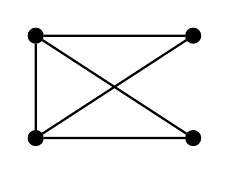
\begin{tikzpicture}[every node/.style={circle,draw=black,fill=black,inner sep=0pt,minimum size=5pt},thick]
\node (A) at (0,1.3) {}; \node (B) at (2,1.3) {}; \node (C) at (0,0) {}; \node (D) at (2,0) {};
\draw (A)--(B) (A)--(C) (A)--(D) (B)--(C) (C)--(D);
\end{tikzpicture}
\caption{A simple graph with four vertices and five edges.}
\end{figure}

The vertices might represent people, towns, tasks or websites. An edge records the relation of interest: friendship, a road, a prerequisite or a hyperlink. A good model makes the question precise. If roads have travel times, use a \emph{weighted graph}; if a connection has a direction, use a \emph{directed graph}; if two towns have several distinct roads between them, use a \emph{multigraph}.

To model the opening question, first choose a travel mode and a destination in the Blue Mountains. For a driving model, let vertices represent road junctions and edges represent road segments; use directed edges for one-way roads. Give each edge an estimated travel-time weight, perhaps for a specified departure time. A journey is then represented by a path, and its total travel time is the sum of its edge weights. The fastest journey is a path of minimum total weight, which need not use the fewest roads or cover the shortest distance.

A different question is how to connect several electricity-network hubs at the lowest total construction cost. Represent the hubs by vertices, possible links by edges, and estimated costs by weights. If the only requirement is to connect every hub without redundant links, the model asks for a minimum spanning tree. This is a deliberately simplified teaching model: real electricity-network design also has to account for reliability, capacity, demand and engineering constraints, among others.

\section{From situation to graph}
A modelling checklist:
\begin{enumerate}
\item Decide what the vertices represent.
\item Decide what an edge means, including whether direction or repetition matters.
\item Add weights or labels only when the question needs them.
\item Check whether the model preserves the feature you want to study.
\end{enumerate}
For a timetable conflict graph, each vertex can represent a class and an edge can join two classes that share students. A proper colouring then assigns times so that conflicting classes get different times.

\section{When are two drawings the same graph?}
The same graph can be drawn with vertices in different places and edges bent or straight. Two graphs are \emph{isomorphic} if there is a bijection between their vertices such that two vertices are adjacent exactly when their corresponding vertices are adjacent. In other words, the names and layout may change, but the connection pattern does not.

\begin{example}
A triangle drawn as a triangle and the same three vertices drawn at the corners of a curved shape are isomorphic: every pair is joined. By contrast, a three-vertex path is not isomorphic to a triangle, because the path has two edges and the triangle has three.
\end{example}

To show two graphs are not isomorphic, find a property preserved by isomorphism that differs: number of vertices, number of edges, degrees, number of components, or cycle lengths. Matching these properties does not by itself prove isomorphism; a valid vertex correspondence must preserve every edge.

\section*{Exercises}
\begin{enumerate}
\item Draw a graph for five people where an edge means ``has exchanged a book with''. What information is lost if you draw only whether an exchange has ever happened?
\item A one-way social-media follow relation is modelled by a graph. What kind? How might you model how many messages were exchanged?
\item Can two non-isomorphic graphs have the same number of vertices and edges? Draw an example on four vertices.
\item A school wants to schedule exams with no student required to sit two exams at once. Describe a graph model and explain what a colouring represents.
\end{enumerate}
